\documentclass{article}[18pt]
\usepackage{../../../../../format}
\lhead{CSys - Databases}
\usepackage[cache=false]{minted}

\begin{document}
\begin{center}
\underline{\huge SQL I}
\end{center}
\section{Database languages}
\begin{itemize}
	\item A good database language should allow users to:
	\begin{itemize}
		\item Create the database, define relation structures
		\item Perform basic data management
		\item Perform simple and complex queries
	\end{itemize}
	\item All these tasks with minimal user effort!
	\begin{itemize}
		\item Syntax/command structure should be easy to learn
		\item Users should concentrate on which queries to make (not how they are implemented)
	\end{itemize}
	\item The language should be portable:
	\begin{itemize}
		\item Conform to a recognized standard
		\item We can use the same language with many DBMS's
	\end{itemize}
	\item SQL: (structured query language)
	\begin{itemize}
		\item The most common database language
		\item simple syntax/ easy to learn and use
		\item It has two components: DDL \& DML
	\end{itemize}
	\item Data Definition Language (DDL)
	\begin{itemize}
		\item Allows users to define the database
		\item Define the schema for each relation (attributes/types)
		\item Define the domain of each attribute
		\item Specify integrity constraints
	\end{itemize}
	\item Data Manipulation Language (DML)
	\begin{itemize}
		\item Allows users to insert/update/delete/retrieve data from the DB
		\item Query Language: the part of the DML that involves data retrieval
	\end{itemize}
\end{itemize}
\section{Two types of query languages}
\begin{itemize}
	\item SQL: formal definition of a new relation from existing relations in the DB
	\item Relational algebra: specifies how to build a new relation from existing relations in the DB
	\item Their place in the big picture
\end{itemize}
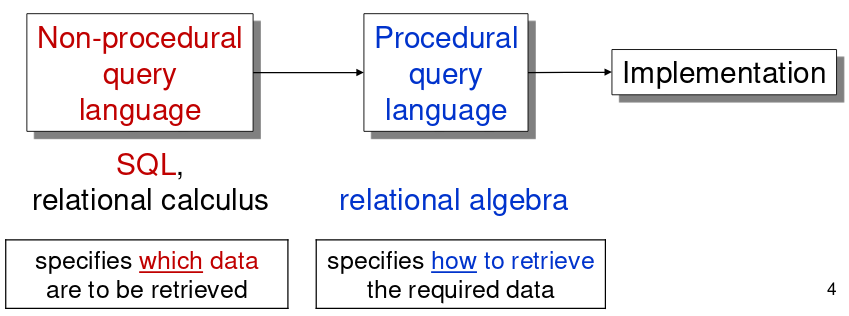
\includegraphics[scale=0.7]{overview}
\section{Writing SQL statements}
\begin{itemize}
	\item SQL statements consist of:
	\begin{itemize}
		\item Reserved words: a fixed part of SQL
		\item User defined words: made up by the user
	\end{itemize}
	\item SQL Statements
	\begin{itemize}
		\item Case insensitive (both upper/lower case)
		\item Except for literal character data (i.e. data entries)
	\end{itemize}
	\item SQL is free-format
	\begin{itemize}
		\item Parts of statements do not have to be written in specific locations on the screen
	\end{itemize}
	\item However:
	\begin{itemize}
		\item More readable with systematic indentation and lineation
		\item Each clause should begin on a new line
		\item Start of a clause should line up with the start of other clauses
		\item If a clause has several parts, they should each appear on separate lines and be indented under the start of clause
	\end{itemize}
\end{itemize}
\section{Data Manipulation Language (DML)}
\begin{itemize}
	\item We mainly look at DML aspects of SQL
	\item To create a database in MySQL
	\begin{itemize}
		\item either use DDL command
		\item or just use the interactive tools of phpMyAdmin 
	\end{itemize}
	\item Main statements of interest in DML:
	\begin{itemize}
		\item SELECT - to query data in the database
		\item INSERT - To insert new data into an existing table
		\item UPDATE - To update data in an existing table
		\item DELETE - To delete data from an existing table
	\end{itemize}
\end{itemize}
\section{Writing SQL commands}
\begin{itemize}
	\item Literals (character data/ numericals) are constants used in SQL statements
	\item All non numeric literals must be enclosed in single quotes
	\item All numeric literals must not be enclosed in quotes
	\item Notation:
	\begin{itemize}
		\item UPPER-case letters represent \textbf{reserved} words
		\item lower-case letters represent \textbf{user-defined} words
		\item a vertical bar (|) indicates a choice among \textbf{alternatives}
		\item curly braces $\{a\}$ indicate a required element
		\item square braces [a] indicate an optional element
		\item ellipsis (...) indicates optional repetition (0 or more)
	\end{itemize}
\end{itemize}
\section{Examples of syntax}
All examples are based on the following tables:
\begin{center}
	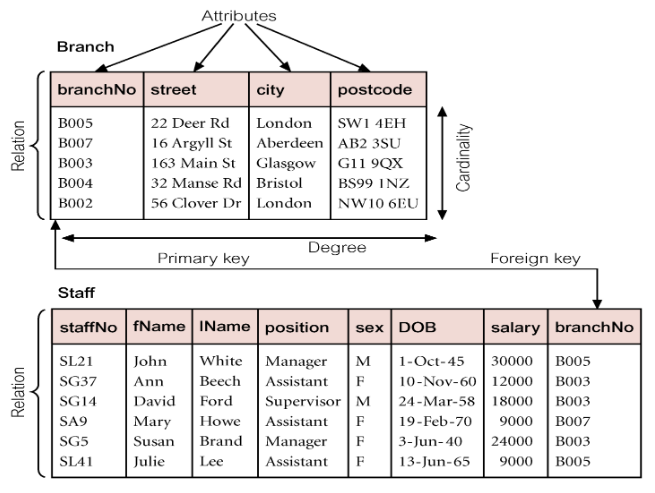
\includegraphics[scale=0.7]{example}
\end{center}
\subsection{Simple queries}
The sequence of processing in a SELECT-FROM-WHERE statement is:
\begin{itemize}
	\item SELECT: specifies which columns are to appear in the output
	\item FROM: specifies the table or tables to be used
	\item WHERE: filters the rows subject to some condition
	\begin{itemize}
		\item GROUP BY: forms groups of rows with the same column value
		\item HAVING: filters the groups subject to some condition
		\item ORDER BY: specifies the order of the output
	\end{itemize}
\end{itemize}
\begin{center}
	{\Large SELECT and FROM are mandatory}
\end{center}
\subsection{Syntax}
\begin{minted}{sql}
SELECT [ALL|DISTINCT] column1[,column2,column3,...]
FROM table1[,table2,table3,...]
[WHERE 'conditions']
[GROUP BY 'column-list']
[HAVING 'conditions']
[ORDER BY 'column-list' [ASC|DESC]]
\end{minted}
Example:
\begin{minted}{sql}
SELECT staffNo, fName, IName, position, sex, DOB, salary, branchNo FROM staff;
\end{minted}
\begin{itemize}
	\item The above statement will select the (whole) specified columns from the staff table
\end{itemize}
Note that if you want to place more queries at once, remember to put a semicolon at the end of each SQL statement. The ; indicates that your SQL statement has finished and the next one can start
\section{SELECT}
\subsection{Example 1}
\begin{itemize}
	\item \textit{List full details of all staff (all columns, all rows)}
	\begin{minted}{sql}
SELECT staffNo, fName, IName, position, sex, DOB, salary, branchNo FROM Staff
	\end{minted}
	\item Alternative
	\begin{minted}{sql}
SELECT * FROM Staff
	\end{minted}
\end{itemize}
\subsection{Example 2}
\textit{Produce a list of salaries for all staff, showing only: staff number, first name, last name and salary}
\begin{minted}{sql}
SELECT staffNo, fName, IName, salary FROM Staff 
\end{minted}
This command creates a new table from the table Staff containing the designated columns in the specified order.\\
The rows are NOT ordered
\subsection{Example 3}
\textit{Produce a list of monthly salaries for all staff, showing only staff number, first name, last name and \textbf{monthly salary}}
\begin{minted}{sql}
SELECT staffNo, fName, IName, salary/12 FROM Staff
\end{minted}
We can leave the column name blank or use an "AS" clause
\begin{minted}{sql}
SELECT staffNo, fName, IName, salary/12 AS 'Month Salary' FROM Staff
\end{minted}
\section{SELECT \& FROM clause review}
\begin{minted}{sql}
SELECT first_column_name, second_column_name
FROM table_name
WHERE first_column_name>12000
\end{minted}
\begin{itemize}
	\item Next to the SELECT keyword:
	\begin{itemize}
		\item the column name(s) specify which will be returned
		\item as many columns as we like
		\item or * to return all columns
	\end{itemize}
	\item Next to the FROM keyword:
	\begin{itemize}
		\item The table name(s) specifies the table that will be required to retrieve the results
	\end{itemize}
	\item Next to the (optional) WHERE keyword:
	\begin{itemize}
		\item the condition(s) specifies which rows will be returned (filtering the rows)
	\end{itemize}
\end{itemize}
\section{DISTINCT}
\begin{itemize}
	\item In normalized relational tables there are no repeated rows
	\item But the use of SELECT may have duplicate rows
	\begin{minted}{sql}
SELECT propertyNo FROM Viewing
	\end{minted}
\begin{center}
	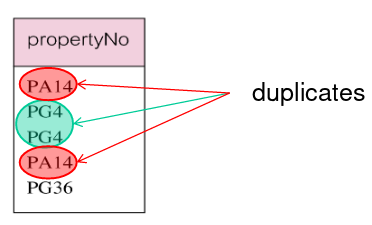
\includegraphics[scale=0.7]{duplicate}
\end{center}
\item Use DISTINCT to eliminate duplicates
\begin{minted}{sql}
SELECT DISTINCT propertyNo FROM Viewing
\end{minted}
\end{itemize}
\subsection{SELECT Statement, Example 4 (DISTINCT)}
List all branch numbers for all branches
\begin{minted}{sql}
SELECT branchNo FROM Staff
\end{minted}
With use of DISTINCT:
\begin{minted}{sql}
SELECT DISTINCT branchNo FROM Staff
\end{minted}
\section{SELECT statement (WHERE)}
\begin{itemize}
	\item We often need to restrict the rows that are retrieved
	\item The WHERE clause is followed by a search conditions (predicates)
	\begin{itemize}
		\item Comparisons: compare values of two expressions
		\item Range
		\begin{itemize}
			\item BETWEEN/NOT BETWEEN
			\item tests whether the values falls within a specified range
		\end{itemize}
		\item Set membership
		\begin{itemize}
			\item IN/NOT IN
		\end{itemize}
		\item Pattern matching
		\begin{itemize}
			\item LIKE/NOT LIKE
		\end{itemize}
	\end{itemize}
\end{itemize}
\section{Range conditions}
\begin{minted}{sql}
SELECT staffNo, salary
FROM staff
WHERE salary BETWEEN 20000 AND 30000
\end{minted}
Is there same as
\begin{minted}{sql}
SELECT staffNo, salary
FROM staff
WHERE salary >= 20000 AND Salary <= 30000
\end{minted}
Note that this is inclusive
\section{Set membership conditions}
\textit{List all managers and supervisors}
\begin{minted}{sql}
SELECT staffNo, fName, IName, position
FROM Staff
WHERE position IN ('Manager','Supervisor')
\end{minted}
This is just to make syntax nicer, it is equivalent to:
\begin{minted}{sql}
SELECT staffNo, fName, IName, position
FROM Staff
WHERE position='Manager' OR position='Supervisor'
\end{minted}
\section{Pattern matching (LIKE)}
\begin{itemize}
	\item Sometimes we want to search within a string
	\item SQL has two special pattern matching symbols
	\begin{itemize}
		\item \% represents an arbitrary sequence of zero or more characters (called wildcard)
		\item \_ represents an arbitrary single character
	\end{itemize}
	\item LIKE 'H\%' means:
	\begin{itemize}
		\item first character must be H, but the rest can be anything
	\end{itemize}
	\item LIKE 'H\_\_\_' means:
	\begin{itemize}
		\item exactly 4 characters, first character must he H
	\end{itemize}
	\item LIKE '\%e' means:
	\begin{itemize}
		\item any sequence of characters, ending at 'e'
	\end{itemize}
	\item NOT LIKE 'H\%' means:
	\begin{itemize}
		\item The first character can not be 'H'
	\end{itemize}
\end{itemize}
Find all owners with the string 'Glasgow' in their address
\begin{minted}{sql}
SELECT ownerNo, fName, IName, address, telNo
FROM PrivateOwner
WHERE address LIKE '\%Glasgow\%'
\end{minted}
\section{Combining conditions and Boolean Operations}
\begin{itemize}
	\item The logical AND operator:
	\begin{itemize}
		\item both sides of the condition must be true
	\end{itemize}
	\item The logical OR operator:
	\begin{itemize}
		\item at least one of the two sides must be true
	\end{itemize}
	\item They can be used in two (or more) conditions in the WHERE clause
\end{itemize}
\begin{minted}{sql}
SELECT fName, IName, position, salary
FROM staff
WHERE position = 'Manager' OR position='Supervisor
\end{minted}
\begin{minted}{sql}
SELECT fName, IName, position, salary
FROM staff
WHERE salary>=24000 AND title='Manager'
\end{minted}
These two operators can also be used combined
\section{ORDER BY clause}
\begin{itemize}
	\item In the resulting table of a SELECT query the rows are NOT ordered
	\item ORDER BY can be used to sort the rows
	\begin{itemize}
		\item according to the values of a particular set of columns
		\item can be ascending/descending
		\item ordering appears regardless of whether that column appears in the result
	\end{itemize}
\end{itemize}
General format:
\begin{minted}{sql}
SELECT column1
FROM 'list-of-tables'
ORDER BY 'column-list' [ASC|DESC]
\end{minted}
We can also sort according to multiple columns:
\begin{itemize}
	\item first sort according to the first column
	\item among rows with the same value in the first column, sort according to the second column etc
\end{itemize}
\section{Aggregate functions}
Aggregate functions:
\begin{itemize}
	\item Operate on a single column
	\item return a single (numeric) value
\end{itemize}
\begin{center}
	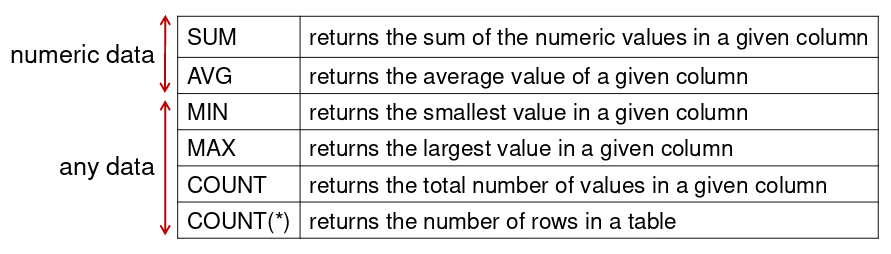
\includegraphics[scale=0.7]{Aggregate}
\end{center}
\subsection{Examples}
\textit{How many properties cost more than £350 to rent}
\begin{minted}{sql}
SELECT COUNT (DISTINCT propertyNo) AS myCount
FROM PropertyForRent
WHERE rent>350
\end{minted}
\section{GROUP BY clause}
\begin{itemize}
	\item Aggregate functions are similar to the totals at the bottom of a report
	\item Often we need also "subtotals" in reports at the bottom of some part of the report
	\item GROUP BY can be used to:
	\begin{itemize}
		\item partition the data into groups
		\item produce a single summary row (e.g. "subtotal") for each group
	\end{itemize}
\end{itemize}
\textit{Find the number of staff working in each branch and sum of their salaries}
\begin{minted}{sql}
SELECT branchNo,
	COUNT(staffNo) AS myCount
	SUM(Salary) AS mySum
FROM staff
GROUP BY branchNo
ORDER BY branchNo
\end{minted}

\end{document}